\section{Conclusion}
\label{sec:conclusion}
In this paper, we propose ZomeFab, a hybrid fabrication method that combines Zometool 
and 3{D} printing to fabricate a large-scale 3{D} objects. 
We aimed to decompose an input 3D object into a inner structure and pieces of outer surfaces. 
By replace the huge inner space with Zometool from 3D printed materials, we can greatly save the cost of 3D printing.
% Compared to print partitioned input mesh directly, the inner structure greatly saves the cost of 3D printing. 
And we retain the fine geometric detail by printing the outer shell with 3D printer.
% The outer surfaces still remain the fine geometric characteristic of 3D printer. 
With the reusability of Zometool, the long-term cost of fabrication is greatly decreased. 
We have demonstrated that our method is able to fabricate large-scale object by physically replicate 5 objects.
% However, Zometool is a complex geometric system which can build thousands of structures. 
% Our method generate a Zometool result which can simply build and also fit in well for outer surface. 
% User can get the pretty well result by using Zomefab.

\subsection{Limitations and Future Work.}
There are many remaining challenges and opportunities for future research on large-scale fabrication.
While our initial unit structure is simple and easy-to-assemble, it's size (4.7cm x 4.7cm x 4.7cm) prevents us to fabricate 3D object with thin structure.
Meanwhile, since Zometool is designed under formal and strict mathematical formulation, the connection between two separated Zometool sub-structure might not exist within the 3D object inner space.
As a result, our method can not fabricate 3D object with two or more parts connected by thin structure that our init unit structure can not fit in.
In the future, we would love to investigate how to shrink the size of the initial unit structure, in order to enable more complicated large-scale 3D object fabrication.
Also, we also interested in analyzing the balance of our Zometool structure, so that we can generate more varieties of 3D objects.
% \subsection{Limitation}
% %Zomefab relied on the input mesh which have the large inner volume and using Zometool as inner structure. The smallest Zometool cube (4.7cm x 4.7cm x 4.7cm) is limited. Therefore, in order to get the initial structure have to make sure input mesh's inner volume must larger than one unit cube. In the future, we can change the unit cube into different and smaller shape to get better structure fitting inside the mesh.
% Though Zomefab can provide a method for user to design the large prototype with 3{D} printing and Zometool. But our method still has some limitations. As three conditions: 

% \subsubsection{Big inner volume} 
% Our initial structure, Zometool-cube, is a 4.7cm x 4.7cm x 4.7cm repeat structure. Therefore, in order to get the initial structure, we have to make sure that the input mesh's inner volume must larger than one unit cube. %(\figname~\ref{fig:limitation}(a))

% \subsubsection{Multiple part of initial structure} 
% Although Zometool have thousands of construct methods, it still has a mathematical model. It means that the construct method is finite. Multiple part of initial structure maybe can't find a Zometool connection path. It will make the balance of structure very dangerous. So we recommend user's input mesh just has single main structure. 
% %(\figname~\ref{fig:limitation}(b))

% \subsubsection{Thin part of input mesh} 
% Our method doesn't have the analysis of balance. 
% %Although the input mesh have a very large inner volume, if the mesh have to rely on the thin part lay on the surface, our system can't ensure the result whether can put on the surface perfectly. 
% Even if the input mesh has a very large inner volume and have to rely on the thin parts which contact on the surface, our method don't have the balance analysis and can't ensure whether the result can put on the surface perfectly. 

%(\figname~\ref{fig:limitation}(a))
%\begin{figure*}[ht]
%\centering
%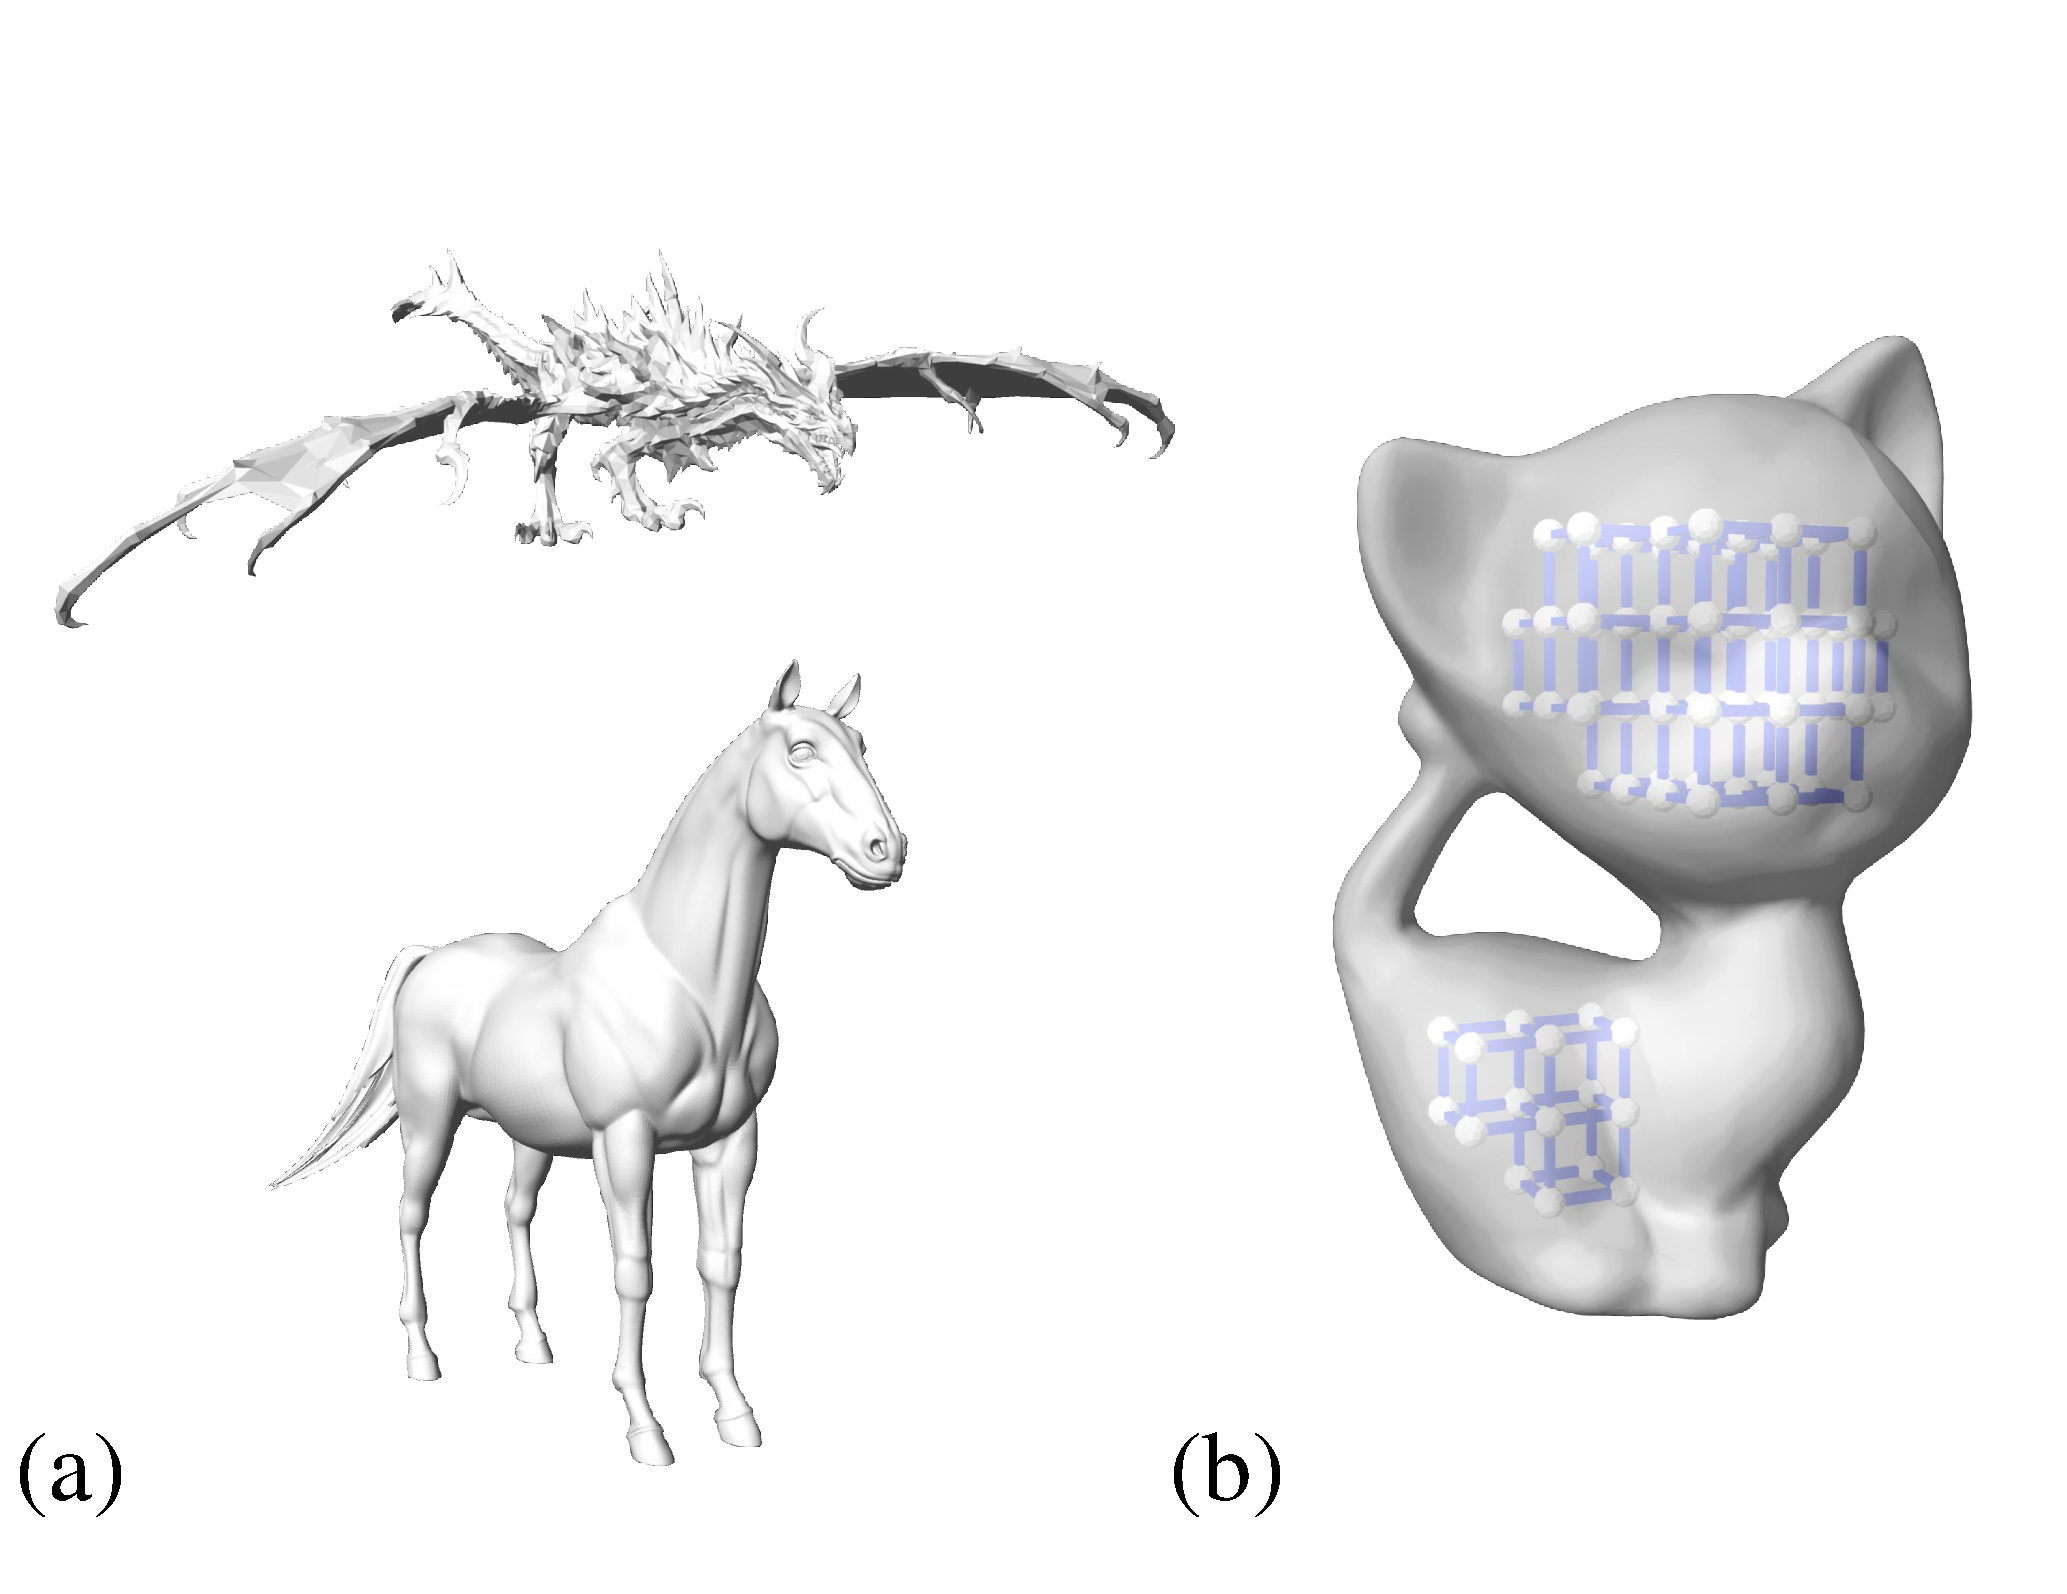
\includegraphics[width=1.0\linewidth]{figs/limitation.pdf} 
%\caption{Our method's limitations. (a) The mesh's inner volume is too small or the %mesh has the thin parts (b) Have multiple parts of initial structure}
%\label{fig:limitation}
%\end{figure*}

% \subsection{Future work}
% In order to handle our method's limitations, we have some following changes for our method:

% \subsubsection{Change the smaller unit shape} 
% Current repeated structure is a little bit bigger for common mesh. To let structure fit inside the mesh better, we have to think if there is another structure that is smaller and better than Zometool-cube.

% \subsubsection{Handle multiple part of initial structure} 
% Lots of mesh don't have a main big volume but have multiple parts which can put Zometool-cube in. One aspect is the balance problem, and the other is our growing tenon's method just can grow out one direction on one piece. We can modify the method to let the different parts of Zometool structures be connected by one printing piece. 

% \subsubsection{Analyze the structure balance} 
% Current method doesn't have balance analysis system. So our input mesh has to find some mesh that has large inner volume for our method. If we have balance analysis, we can analyze whether the structure is safe and modify the energy function of simulated annealing, then our result will be more robust.

